\documentclass{beamer} 
%\documentclass[handout]{beamer} 
\usetheme{Ilmenau}
\usepackage{graphicx,verbatim,hyperref}
\usepackage{textpos}

\usecolortheme{beaver}
\useinnertheme{default}
\setbeamertemplate{itemize item}[triangle]
\setbeamertemplate{itemize subitem}[triangle]
\setbeamertemplate{itemize subsubitem}[circle]
\setbeamertemplate{enumerate items}[default]
\setbeamertemplate{blocks}[upper=block head,rounded]
\setbeamercolor{item}{fg=black}
\usefonttheme{serif} %should allow ccfonts to take effect

\usepackage{cite}
\usepackage{times, verbatim,xcolor,bm}
\usepackage{amsbsy,amssymb, amsmath, amsthm}
\usepackage{booktabs}
%David miller's fonts
	\usepackage[T1]{fontenc}
	\usepackage[boldsans]{ccfonts}
	\usepackage[euler-hat-accent]{eulervm}

\newcommand{\al}{\alpha}
\newcommand{\expect}{\mathbb{E}}
\newcommand{\Bt}{B(\bm{\tau^a})}
\newcommand{\bta}{\bm{\tau^a}}
\newcommand{\btn}{\bm{\tau^{tw}}}
\newcommand{\ga}{\gamma}
\newcommand{\ve}{\varepsilon}
\newcommand{\ta}{\theta}
\newcommand{\de}{\delta}
\newcommand{\ov}{\overline}

\newenvironment{changemargin}[2]{% 
  \begin{list}{}{% 
    \setlength{\topsep}{0pt}% 
    \setlength{\leftmargin}{#1}% 
    \setlength{\rightmargin}{#2}% 
    \setlength{\listparindent}{\parindent}% 
    \setlength{\itemindent}{\parindent}% 
    \setlength{\parsep}{\parskip}% 
  }% 
  \item[]}{\end{list}} 

\begin{document}
\title[Unrecognized States: A Theory of Self-Determination and Foreign Influence\hspace{1.25in}\insertframenumber/\inserttotalframenumber]{Unrecognized States: A Theory of Self-Determination and Foreign Influence}
\author[Kristy Buzard, Benjamin Graham and Ben Horne]{Kristy Buzard, Benjamin Graham and Ben Horne\\ kbuzard@syr.edu}
\date{April 12, 2015}
\maketitle
%\insertpresentationendpage removed b/c of appendix



\section{Overview}
\subsection{Preview}
\begin{frame}
\frametitle{Unrecognized States}
Unrecognized states (URS): control and govern territory, seek recognition
\pause
\begin{itemize}[<+->]
  \item Six current URS more than 20 yrs old (+ Eastern Ukraine)
	\item No explanation in the literature for how this can be a stable outcome
\end{itemize}
\end{frame}


\begin{frame}{What we do}

\pause
We demonstrate unrecognized statehood can be a ``status quo'' outcome
\pause
\begin{itemize}[<+->]
	\item (SPN) Equilibrium in a repeated game
	\item Four players
		\begin{itemize}[<+->]
			\item Home government
			\item Secessionist elite
			\item Patron state
			\item International community
		\end{itemize}
	\item State variable: Status Quo (SQ) payoffs for secessionists
\end{itemize}

\end{frame}



\begin{frame}{The General Idea}

\pause
In each period: secessionists and gov't each choose (simultaneously) among $\left\{\text{Fight, Status Quo, Cede}\right\}$
\pause
		\begin{itemize}
			\item We need SQ to be a stage game best response for both secessionists and gov't
		\end{itemize} 

\pause
\vskip.2in
We add some more realistic elements:
\pause
		\begin{enumerate}[<+->]
			\item Unrecognized status reduces SQ payoffs of secessionists each period
			\item Patron and int'l community can make investments in both actors' payoffs
		\end{enumerate}

\end{frame}


\begin{frame}{Outline of Talk}
\pause
\begin{enumerate}[<+->]
	\item Model
	\item Status quo equilibrium
	\item What we can say about sanctions
	\item Conclusion
\end{enumerate}
\end{frame}



\section{Model}
\subsection{Economic and Political Structure}
\begin{frame}{Timeline}
\pause
\begin{figure}
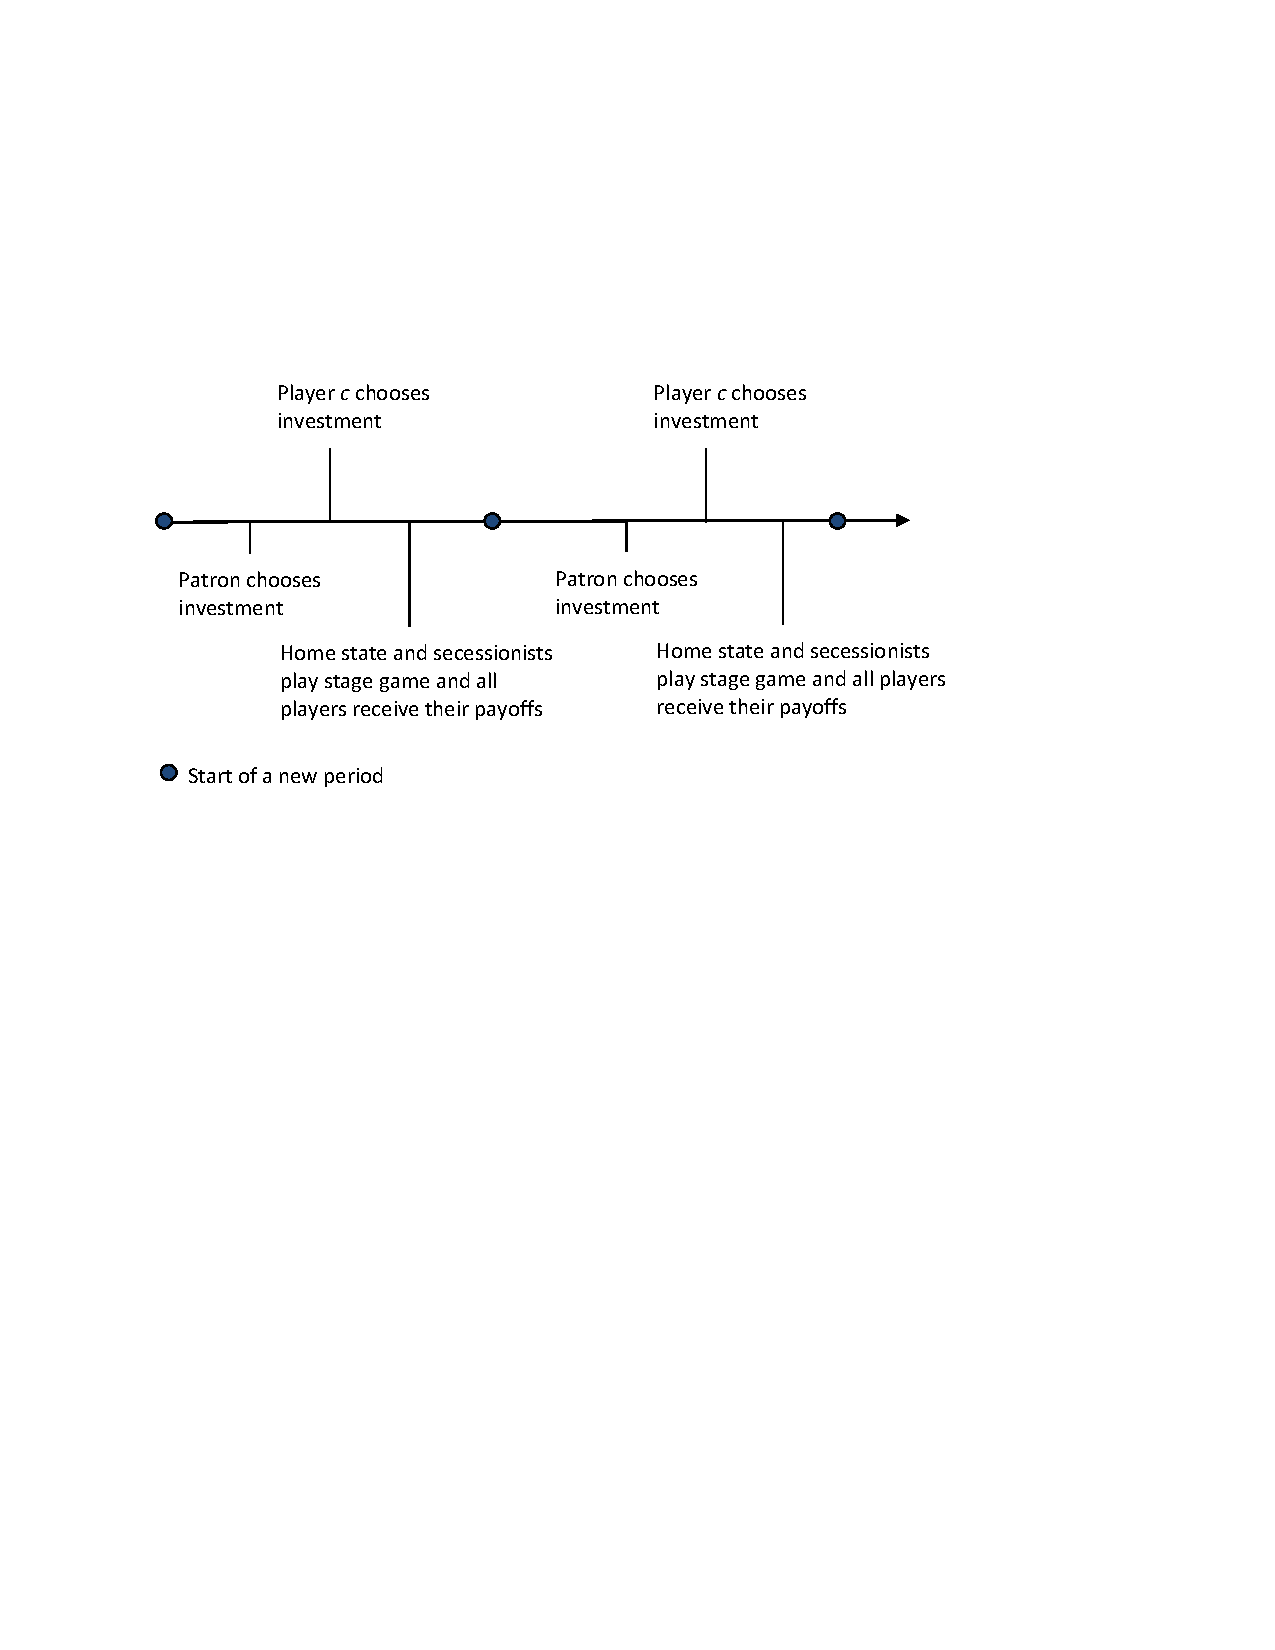
\includegraphics[width=\linewidth,height=\textheight,keepaspectratio]{Timeline2.pdf}
\caption{Timeline}
\end{figure}
\end{frame}


\subsection{The Players}

\begin{frame}{Outside Actors}
	\pause
International community ($c$): desires reunification \\
\pause
Patron ($p$): desires recognized independence
\pause
\begin{itemize}	
	\item Each has preferences that are aligned with one of the home state actors
	\pause
	\item Patron may most prefer SQ; our assumption stacks the deck against us
\end{itemize}

\pause
\vskip.2in
$p$'s per period payoffs: $U_{pt} = -\alpha X + \lambda Y - R_{pt}$ \\
$c$'s per period payoffs: $U_{ct} = \beta X - \nu Y - R_{ct}$
\begin{itemize}
	\item $X=1$ if the secessionists rejoin the home state \\
	\item $Y=1$ if the home state recognizes the secessionists 
\end{itemize}
\end{frame}



\begin{frame}{Home State Actors}
	\pause
Central Government of Home State ($g$): desires reunification \\
\pause
Secessionists ($s$): desire recognized independence
\pause
\begin{itemize}	
	\item Central issue of contention: recognized independence vs. reunification.
\end{itemize}

\pause
\vskip.2in
Assumptions:
\begin{itemize}[<+->]
	\item Issue of status is indivisible, highly valued by both sides
	\item Insufficient credible side payments for easy settlement
\end{itemize}
\end{frame}


\begin{frame}{Stage Game between Home Gov't $\&$ Secessionists}
\pause
	\begin{center}
\begin{tabular}{|  c| c | c | c |} 
\hline
  $g\downarrow$,     $ s\rightarrow$  & Fight & Status Quo &Cede \\ \hline
	Fight & $\omega_{gt}, \omega_{st}$ &$\omega_{gt}, \omega_{st}$&$W_{gt}, L_{st}$ \\ \hline
	Status Quo& $\omega_{gt}, \omega_{st}$& $Q_{gt}, Q_{st}$ &$W_{gt}, L_{st}$ \\ \hline
	Cede&$L_{gt}, W_{st}$& $L_{gt}, W_{st}$ &$Q_{gt}, Q_{st}$ \\ \hline
 \multicolumn{4}{c} {Stage Game Payoffs}\\ 
\end{tabular}
\end{center}
where $\omega_{it} \equiv p_1 \left(W_{it}-\zeta_i\right) + \left(1-p_1\right)\left( L_{it}-\zeta_i\right)$
\begin{itemize}
	\item fixed cost of war $\zeta_i$
	\item probabilities $p_1$ of victory, $1 - p_1$ of loss 
		\begin{itemize}
			\item can also handle non-decisive war
		\end{itemize}
\end{itemize}
and $Q_{st} \equiv Q_{s,t-1} -\mu + R_{pt} - R_{ct}$
\end{frame}


\section{Status Quo Equilibrium}
\subsection{}


\begin{frame}{Main Result}
\begin{beamerboxesrounded}[upper=palette tertiary, shadow=true]{Proposition 1}
  There exists an equilibrium in which the outcome is perpetual unrecognized statehood. The actions in this equilibrium are 
	\begin{enumerate}
		\item $p$ invests to create a buffer of $\frac{\beta}{1-\delta}$ between the payoffs from ceding and the status quo in the first period;
		\item $p$ invests up to $\mu$ each period thereafter to maintain the buffer;
		\item $c$ invests nothing;
		\item both $g$ and $s$ play $Status$ $Quo$ each period.
	\end{enumerate}
	
\end{beamerboxesrounded}
\end{frame}

\begin{frame}{Proposition 1 Continued}
\pause
  The following are sufficient conditions for the equilibrium:
	\begin{enumerate}[<+->]
		\item \textit{For both $g$ and $s$, $Q_{it} \geq L_{it} \ \forall t$.}

		\item \emph{For both $g$ and $s$, $\frac {Q_{it}}{1-\delta} \geq  -\zeta_i+\frac{W_{it}(p_1) + L_{it}(1-p_1)}{1-\delta} \ \forall t$.}

\item \textit{$\alpha \geq \beta$: reunification is more important for $p$ to avoid than for $c$ to achieve.}

\item  \textit{$\nu\cdot p_{1s} \geq \lambda \cdot p_{1s} + \mu + \beta$: recognition of $s$ is more important for $c$ to avoid than for $p$ to achieve.}

\item  \textit{$B_{p1} \geq\frac{\beta}{1-\delta} - \left(q_{s1} - l_{s1} \right)$: the patron can afford to deter player $c$ from inducing reunification at the beginning of the game.}

\item \textit{$B_{pt} \geq \mu, \ \forall t>1$: the patron can afford to pay to maintain the status quo.}
	\end{enumerate}
\end{frame}

\section{Sanctions}
\begin{frame}{Sanctions (I)}
\begin{beamerboxesrounded}[upper=palette tertiary, shadow=true]{Proposition 2}
  Assume the conditions of \emph{Proposition 1} hold in the absence of sanctions and that sanctions affect only player $s$'s Status Quo payoffs. In order for sanctions to lead to ceding by the secessionists, the following are required:
	\pause
	\begin{enumerate}[<+->]
\item The patron must be unable or find it not worthwhile to invest the additional amount now required to maintain the status quo.

\item The patron must be unable or find it not worthwhile to invest to instigate fighting by the secessionists.

\item The continuation value from SQ must fall below that from Cede before it falls below that from Fight.
\end{enumerate}

\end{beamerboxesrounded}

\end{frame}

\begin{frame}{Sanctions (II)}
\begin{beamerboxesrounded}[upper=palette tertiary, shadow=true]{Proposition 3}
  Assume the conditions of \emph{Proposition 1} hold in the absence of sanctions and that sanctions affect both player $s$'s status quo payoffs and its military capabilities. \\
	\pause
	The parameter space over which a war will be initiated by the home state is increasing in the magnitude of the sanctions' impact on the secessionists' military capabilities.
\end{beamerboxesrounded}

\end{frame}


\section{Conclusion}
\subsection{}
\begin{frame}{Conclusion}
\begin{itemize}[<+->]
	\item We present a unified four-player framework for analyzing unrecognized statehood and its alternatives
	\item We show unrecognized statehood can emerge in equilibrium even when it is a terrible outcome for all involved
		\begin{itemize}
			\item Unfortunately, it is not difficult to imagine Eastern Ukraine on our list of URS in 20 years
		\end{itemize}
	\item The model demonstrates why sanctions may be counterproductive and suggests that positive inducements may be more productive
\end{itemize}

\end{frame}


\end{document}